\documentclass{amsart}
\usepackage{graphicx}
\graphicspath{{./}}
\usepackage{hyperref}
\usepackage{csvsimple}
\usepackage{longtable}
\usepackage{lscape}
\usepackage{epigraph}
\title{Ethnicity Effects on Trust From Family to the World: Universal Human Nature Feature}
\author{Zulfikar Moinuddin Ahmed}
\date{\today}
\begin{document}
\maketitle

\section{Graphical Evolution in Emotional Distance}

We place ethnicity-grouped trust levels for family, known, neighborhood, strangers, people of other nationality in order.  Our focus is visual geometry in order to formulate a {\em dynamic model of trust as a function of distance} with World Values Survey data and without further measurements.

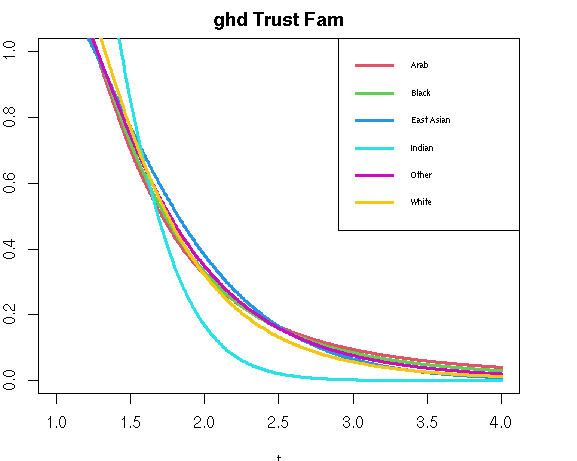
\includegraphics[scale=0.8]{trfam_fitted.png}

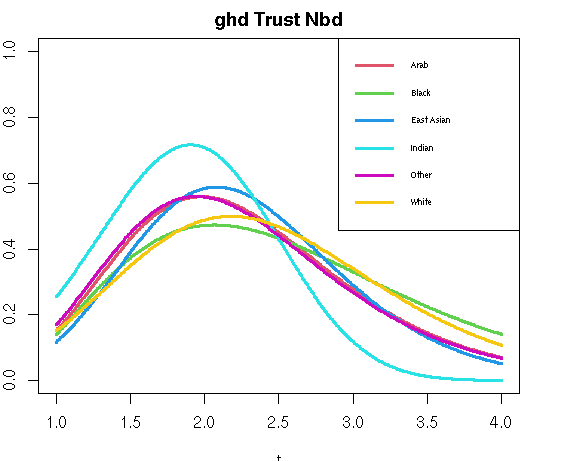
\includegraphics[scale=0.8]{trnbd_fitted.png}

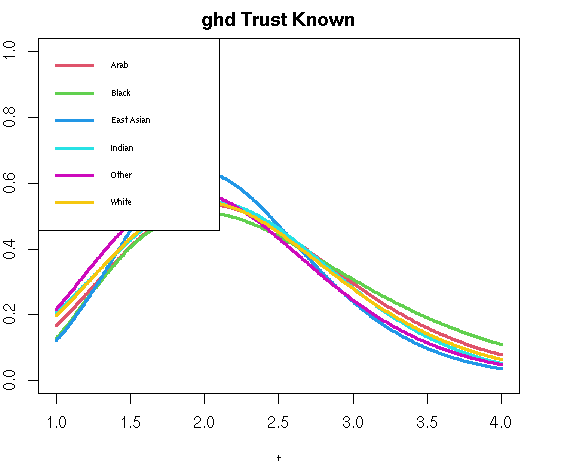
\includegraphics[scale=0.8]{trknown_fitted.png}


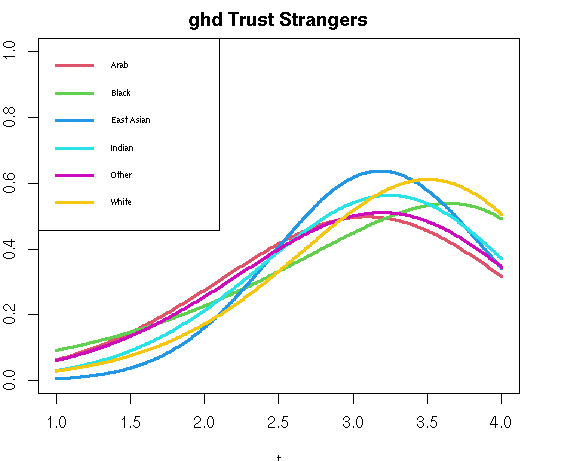
\includegraphics[scale=0.8]{trstrangers_fitted.png}

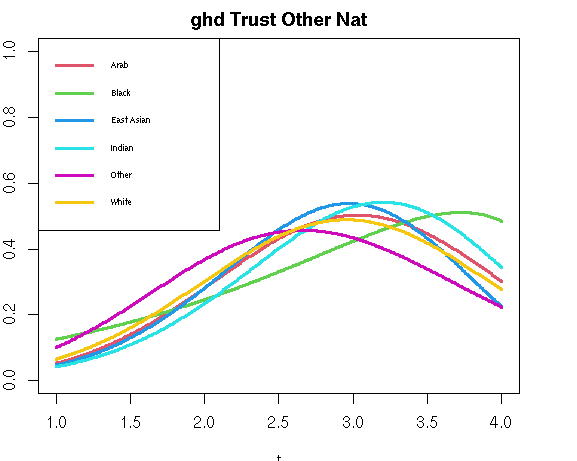
\includegraphics[scale=0.8]{trothernat_fitted.png}

\section{Human Race Emotional Distance-Trust Model Proposal}

We propose a serious scientific model for trust levels of the entire human race based on emotional distance that is precise.  The sequence of plots of data in the last section tells us that here a quantitative model can succeed simply by {\em interpolation} of densities.  Such a model would be guaranteed to calibrate well to the measured data.  Continuous interpolation provides us with {\em predictions} of the model that could be tested later on.  The reason even without extensive testing we can be fairly confident that our model will be accurate is the strong clustering of trust level curves across all ethnicities.  Thus trust level is definitely a Human Nature variable.

I won't go into the extensive empirical work that has already been done on this problem at the {\em individual level} since our domain is not individual level but {\em human race level}.  In other words we are interested in {\em evolution of Barndorff-Nielsen Densities} as a deterministic function of emotional distance.  We are almost guaranteed to succeed in producing an extremely accurate model, and one of the central models on Human Nature Psychology on one of the most important dimensions of Human Life on Earth.

\section{Interpolation of Barndorff-Nielsen Theta Parameters}

Our approach of reducing all the curves to Barndorff-Nielsen densities allow us to evade complex strategies for modeling to that of interpolation.

We will refer to Barndorff-Nielsen parameters as $\theta$.  
\begin{equation}
\theta = (\lambda, \mu, \sigma, \gamma, \bar{alpha}).
\end{equation}

We will then consider five states, (family, known, neighbor, stranger, foreigner).  It will be convenient to refer to these as $s_1,\dots,s_5$ denoting states.  We let
\[
\theta_j = \theta_{s_j}
\]
This means that the {\\em estimated $\theta$ for state $s_j$ is mapped to $\theta_j$.}



We will hypothesize a continuous parameter $x$ representing emotional distance.

We will associate five real values $x_1,\dots, x_5$ to (family, known, neighbor, stranger, foreigner); the determination of these real values is part of our solution.

Then we will produce a smooth real curve $\theta(x) \in \mathbf{R}$ such that 
\[
\theta(x_j) = \theta_j.
\]

With this notation, the problem we have can be reduced to seeking a smooth functional form $\theta(x)$ that interpolates the relevant $\theta_j$ and we have flexibility in choice of $x_j\in\mathbf{R}$.

Then we want to declare the $\theta(x)$ with $x \in [1,5]$ as the parameters of Barndorff-Nielsen densities.

A parsimonious smooth path $\theta(x)$ is our scientific model of {\em Trust in Human Race}.

\section{Problem in Paradise}

We turn now to an example for just the White people.  This is the problem of degeneracy, where we suspect that the parameters estimated, $\theta_q$ are not the ones we want and another set of parameters $\theta_q'$ that are more appropriate will produce at least as good results as $\theta_q$.

Let us illustrate this with actual data.

% latex table generated in R 4.0.3 by xtable 1.8-4 package
% Tue May 18 08:35:42 2021
\begin{table}[ht]
\centering
\begin{tabular}{rrrrrr}
  \hline
 & lambda & mu & sigma & gamma & alpha.bar \\ 
  \hline
family/s1 & -5.19 & 0.00 & 0.32 & 1.18 & 1.99 \\ 
  known/s2 & -13.41 & 0.00 & 0.64 & 2.22 & 8.37 \\ 
  neighbor/s3 & -12.29 & 0.00 & 0.69 & 2.44 & 8.08 \\ 
  stranger/s4 & -61.92 & 10.73 & 0.00 & -7.41 & 39.68 \\ 
  foreigner/s5 & -821.70 & 0.27 & 0.97 & 2.69 & 500.00 \\ 
   \hline
\end{tabular}
\end{table}

As you can see here clearly, $s_4$ is anomalous here in parameter estimation.

\section{Analogy with Quant Models in Finance}

I am an experienced Finance Quant and began my career at Lehman Fixed Income Derivatives in 1995.  The above setup is a Quant Setup and so I can guarantee that the problems can be resolved in a few weeks of effort.  I do not expect extraordinary difficulties here.  Quants have sufficient tools to ensure success.

\section{Expected Characteristics of A Scientific Theory of Trust}

The approach we are taking leads to a deterministic exact model for {\em probability density of trust levels in a continuous parameter from very close to very distant}.  We will be able to be almost exact for the Barndorff-Nielsen density parameters $\theta(x)$ but of course that is all that is determined.  A given person's trust characteristics will have a probability density and we can sample randomly from that distribution for any emotional distance.  This is intrinsically stochastic.

An analogy might help.  In the relationship between Brownian motion and heat equation, the density $p_t(x,y)$ or the heat kernel evolves by an exact partial differential equation.  But of course individual particles follow a stochastic process.  Our trust model will maintain this sort of stochasticity for individuals.  

At this point, we would distrust any model that is not stochastic in this space.  We have strong reasons for this.  In other words, we would be quite skeptical about trust level models that are deterministic.  Why?  Well the universality of some of these densities are probabilistic regularity.  Natural phenomena do not give us examples where one can be deterministic at the individual level with sort of mixing.  We will return to these questions in the future.  We believe the stochasticity is part of Human Nature.

\section{Tinkering and Manual Adjustments}

I adjusted the code for tinkering with constraints to produce parameters for $s_4$ that are more reasonable.  This tinkering is part of scientific work which may or may not lead to review.  Since I don't have deep experience with the parameter sweeping of $\theta$ this tinkering cannot be avoided.  After some tinkering I obtain much more sensible vector for $s_4$.

% latex table generated in R 4.0.3 by xtable 1.8-4 package
% Tue May 18 12:46:25 2021
\begin{table}[ht]
\centering
\begin{tabular}{rrrrrr}
  \hline
 & lambda & mu & sigma & gamma & alpha.bar \\ 
  \hline
family/s1 & -5.191 & 0.000 & 0.320 & 1.180 & 1.986 \\ 
  known/s2 & -13.409 & 0.000 & 0.637 & 2.219 & 8.372 \\ 
  neighbor/s3 & -12.288 & 0.000 & 0.695 & 2.439 & 8.083 \\ 
  stranger/s4 & -89.162 & 0.001 & 0.852 & 3.429 & 400.000 \\ 
  foreigner/s5 & -821.704 & 0.272 & 0.973 & 2.687 & 500.000 \\ 
   \hline
\end{tabular}
\end{table}
\pagebreak

Now for those who are unaccustomed to scientific work, why would I even give up least square error and do what seems like arbitrary constraints?

I'll tell you.  You see the $\sigma$ column?  You see how the $\sigma=0.85$ falls in line with the others?  We love that. The $\bar{\alpha}$ we constrained to 400 so it's in line.  

Now we can use the same constraints to re-estimate $\theta_5$.  

% latex table generated in R 4.0.3 by xtable 1.8-4 package
% Tue May 18 12:53:21 2021
\begin{table}[ht]
\centering
\begin{tabular}{rrrrrr}
  \hline
 & lambda & mu & sigma & gamma & alpha.bar \\ 
  \hline
family/s1 & -5.191 & 0.000 & 0.320 & 1.180 & 1.986 \\ 
  known/s2 & -13.409 & 0.000 & 0.637 & 2.219 & 8.372 \\ 
  neighbor/s3 & -12.288 & 0.000 & 0.695 & 2.439 & 8.083 \\ 
  stranger/s4 & -89.162 & 0.001 & 0.852 & 3.429 & 400.000 \\ 
  foreigner/s5 & -99.886 & 0.001 & 0.967 & 2.961 & 400.000 \\ 
   \hline
\end{tabular}
\end{table}

Now this is looking better for a model.   

\section{Subproblem: Transform Data For Univariate Linear Fits}

We want to consider the transformation
\[
\tau: \mathbf{R}^5 \rightarrow \mathbf{R}^5
\]
such that $\tau(\theta_1),\dots, \tau(\theta_5)$ have the property that their components can be placed on a univariate line.

In other words we want the situation where there exists $t_0<t_1<\cdots<t_4$ and real constants $a_1, a_2, \dots, a_5$ and $b_1,b_2,\dots,b_5$ for which the following hold:
\[
(\tau_j)_r = b_r + a_r t_r
\]
The key point is that the {\em time points} $t_0<\cdots<t_4$ are shared across the univariate linear fits.

\section{An Analogue of EM Algorithm}

We would like an algorithm that fits $(a_1,\dots,a_5,b_1,\dots,b_5, t_0,t_1,t_2,t_3,t_4)$ by an iterative algorithm where the $a$ and $b$ are estimated separately from the $(t_0,t_1,\dots,t_4)$.  

Given $(t_0,\dots,t_4)$ we can just use five univariate linear regressions to estimate $a$ and $b$.  

The nontrivial part is to determine optimal $(t_0,t_1,\dots,t_4)$ given $a$ and $b$.

Then we iterate between finding optimal parameters in each group until there is some convergence.

So our major task is to produce a solution to the second part, of determining $(t_0,\dots,t_4)$.

We can have a separate module for transformation $\tau$.

If we do this, we are optimistic that some reasonable loss function will be small and then all the parameters will be part of our scientific model.  In particular we will {\em interpret} $(t_1-t_0,\dots,t_4-t_3)$ as exact emotional distances between the states $s_1,\dots,s_5$ in the actual data.

\section{Trials and Tribulations of Unorthodox Algorithms}

\begin{verbatim}
# determine t_1, t_2, t_3, t_4 assuming t_0=0

adjust_times<-function( abparams, t0, data ){
  a<-abparams[1:5]
  b<-abparams[6:10]
  objective<-function( t ){
    q <- matrix( 0, nrow=length(t)+1, ncol=5)
    tp<-c(0,t)
    for ( r in 1:5 ){
      q[,r] <- a[r] + b[r]*tp[r]
    }
    error <- 0
    for (r in 1:5){
      de <- norm( data[,r] - q[,r], type="2")
      error <- error + de
    }
    print(error)
    error
  }
  res <- optim( t0, objective, method="Nelder-Mead")
  list(t=res$par, error=res$value )
}

adjust_abs <- function( t, data) {
  as <- rep(0,5)
  bs <- rep(0,5)
  tp <- rep(0,5)
  tp[2:5] <- t 
  for (r in 1:5){
    y<-data[,r]
    mod<-lm(y~ tp )
    as[r] <- coef(mod)[2]
    bs[r] <- coef(mod)[1]
  }
  out<-c(as,bs)
  out
}

det.trust.pars<-function(data){
  error <- 1e8
  t0<-1:4
  ab <- adjust_abs(t0, data)
  t <- t0
  while ( error > 0.001){
    w <- adjust_times( ab, t, data)
    t <- w$t
    ab <- adjust_abs( t, data)
    error <- w$error
  }
  list(ab=ab,t=t)
}
\end{verbatim}


\section{Fit R-squared does improve with moving times around}

Warning:  There are errors in this code that I wish to preserve.  See later sections for fixes.  The errors are important to me.

\begin{verbatim}
# determine t_1, t_2, t_3, t_4 assuming t_0=0

adjust_times<-function( abparams, t0, data ){
  a<-abparams[1:5]
  b<-abparams[6:10]
  objective<-function( t ){
    q <- matrix( 0, nrow=length(t)+1, ncol=5)
    tp<-c(0,t)
    for ( r in 1:5 ){
      q[,r] <- a[r] + b[r]*tp[r]
    }
    error <- 0
    for (r in 1:5){
      de <- norm( data[,r] - q[,r], type="2")
      error <- error + de
    }
    error
  }
  print('opt done')
  res <- optim( t0, objective, method="Nelder-Mead")
  list(t=res$par, error=res$value )
}

adjust_abs <- function( t, data) {
  as <- rep(0,5)
  bs <- rep(0,5)
  tp <- rep(0,5)
  tp[2:5] <- t 
  for (r in 1:5){
    y<-data[,r]
    mod<-lm(y~ tp )
    as[r] <- coef(mod)[2]
    bs[r] <- coef(mod)[1]
  }
  out<-c(as,bs)
  out
}

det.trust.pars<-function(data){
  error <- 1e8
  t0<-1:4
  ab <- adjust_abs(t0, data)
  t <- t0
  count<-0
  while ( error > 10  & count < 200){
    w <- adjust_times( ab, t, data)
    t <- w$t
    ab <- adjust_abs( t, data)
    error <- w$error
    print(count)
    count<-count+1
  }
  list(ab=ab,t=t)
}
\end{verbatim}

I was not sure that moving around t will actually do anything to quality of univariate linear fits.  I just discovered they do make small improvements.  In other words, our code is producing some results that make a difference in the problem.

% latex table generated in R 4.0.3 by xtable 1.8-4 package
% Tue May 18 16:50:13 2021
\begin{table}[ht]
\centering
\begin{tabular}{rrr}
  \hline
 & fixed & var \\ 
  \hline
1 & 88.54 & 89.12 \\ 
  2 & 75.00 & 76.94 \\ 
  3 & 84.91 & 82.03 \\ 
  4 & 76.88 & 72.02 \\ 
  5 & 86.83 & 87.26 \\ 
   \hline
\end{tabular}
\end{table}

\section{Another Pass With Better Results}

\begin{verbatim}
# determine t_1, t_2, t_3, t_4 assuming t_0=0

adjust_times<-function( abparams, t0, data ){
  a<-abparams[1:5]
  b<-abparams[6:10]
  objective<-function( t ){
    q <- matrix( 0, nrow=length(t)+1, ncol=5)
    tp<-c(0,t)
    for ( r in 1:5 ){
      for (s in 1:length(tp)){
        q[s,r] <- b[r] + a[r]*tp[s]
      }
    }
    error <- 0
    for (r in 1:5){
      de <- norm( data[,r] - q[,r], type="2")^2
      error <- error + de
    }
    error<-sqrt(error)
    print(error)
    error
  }
  print('opt done')
  res <- optim( t0, objective, method="Nelder-Mead")
  list(t=res$par, error=res$value )
}

adjust_abs <- function( t, data) {
  as <- rep(0,5)
  bs <- rep(0,5)
  tp <- rep(0,5)
  tp[2:5] <- t 
  for (r in 1:5){
    y<-data[,r]
    mod<-lm(y~ tp )
    as[r] <- coef(mod)[2]
    bs[r] <- coef(mod)[1]
  }
  out<-c(as,bs)
  out
}

det.trust.pars<-function(data){
  error <- 1e8
  t0<-1:4
  ab <- adjust_abs(t0, data)
  t <- t0
  count<-0
  while ( error > 10  & count < 200){
    w <- adjust_times( ab, t, data)
    t <- w$t
    ab <- adjust_abs( t, data)
    error <- w$error
    print(count)
    count<-count+1
  }
  list(ab=ab,t=t)
}
\end{verbatim}

This code is better with rows 2 and 3 swapped!

% latex table generated in R 4.0.3 by xtable 1.8-4 package
% Tue May 18 18:06:02 2021
\begin{table}[ht]
\centering
\begin{tabular}{rrr}
  \hline
 & fixed & var \\ 
  \hline
1 & 90.53 & 99.84 \\ 
  2 & 75.00 & 93.34 \\ 
  3 & 79.10 & 74.50 \\ 
  4 & 70.61 & 75.82 \\ 
  5 & 87.26 & 99.95 \\ 
   \hline
\end{tabular}
\end{table}

Here we begin to see improvements.  The time estimate is the following
\begin{verbatim}
> out$t
[1] 1.089953 1.113365 3.796915 3.823299
\end{verbatim}
This is {\em very important}.  Here $t_0=0$ and the spacing is unequal.



\section{Expected Solution}

We expect to produce $(a_1,\dots,a_5,b_1,\dots,b_5,t_1,t_2,t_3,t_4)$ such that 
\[
\tau^r(t) = b_r + a_r t
\]
fits the $\tau = \log(\theta)$ dataset.  The parameters $t_1,\dots, t_4$ control the emotional distance from $\theta[1,]$.  We've shown how to calibrate the model partially.

\section{What is Clear}
It is clear already for example from the joint $R^2$ above that there exists a $t\in \mathbf{R}$ parametrized Barndorff-Nielsen densities $\delta(x, \theta(t)) = \delta( x,exp(\tau(t))$ where $\tau(t) = \tau(t; a_1, \dots, a_5, b_1, \dots, b_5, t_1,\dots, t_4)$ and this has a simple form such that these parametrises trust at emotional distance $t$ for the entire human race.  It is clear that the calibration will produce good fit. 

Therefore we can see that Trust at the Human Race level is governed by a smooth family of (Barndorff-Nielsen) Levy Processes that fit measurements quantitatively well.

This is a continuous parameter stochastic model of trust whose dynamical interpretation is clear from Levy Process Theory.

\section{Trust Parameter R-Squares}

\begin{verbatim}
vt.rsq<-rep(0,5)
ft.rsq<-rep(0,5)
t5<-rep(0,5)
t5[2:5]<-out$t
t50<-1:5
out<-det.trust.pars( log(abs(wtt2)+0.1))
for (k in 1:5){vt.rsq[k]<-summary(lm( log(abs(wtt2[,k])+0.01)~t5 ))$r.squared}
for (k in 1:5){ft.rsq[k]<-summary(lm( log(abs(wtt2[,k])+0.01)~t50 ))$r.squared}
xtable(data.frame(fixed=ft.rsq*100,var=vt.rsq*100))

> out$t
[1] 1.079613 1.111313 3.787916 3.817898
\end{verbatim}

% latex table generated in R 4.0.3 by xtable 1.8-4 package
% Tue May 18 18:58:42 2021
\begin{table}[ht]
\centering
\begin{tabular}{rrr}
  \hline
 & fixed & var \\ 
  \hline
1 & 90.53 & 99.84 \\ 
  2 & 75.00 & 93.40 \\ 
  3 & 79.24 & 74.57 \\ 
  4 & 70.63 & 75.73 \\ 
  5 & 87.24 & 99.95 \\ 
   \hline
\end{tabular}
\end{table}

We're not going to be getting anything vastly better for $s_3,s_4$ in actual Nature data.  What I do want to emphasise is that this is more than good enough to justify our model and that closeness of $t$ for strangers and foreigners as well as neighbors and people we know compared to the vast separation of the two is most likely {\em important for Nature} and that is why they occur.  You see, I would have no idea that anything but equal spacing is appropriate but estimation gives us these strange $t_2,t_3,t_4,t_5$ and this is a {\em scientific discovery} about emotional distances.

\section{Failure Of Method For East Asians}

The problem here has some delicate issues that I am not clear about yet.  

The repetition of the successful method produces a failure for East Asians.

% latex table generated in R 4.0.3 by xtable 1.8-4 package
% Tue May 18 20:14:36 2021
\begin{table}[ht]
\centering
\begin{tabular}{rrr}
  \hline
 & fixed & var \\ 
  \hline
1 & 91.35 & 98.60 \\ 
  2 & 18.85 & 12.47 \\ 
  3 & 0.10 & 0.47 \\ 
  4 & 84.49 & 69.47 \\ 
  5 & 87.67 & 86.91 \\ 
   \hline
\end{tabular}
\end{table}

We will investigate in the future.  Here $s_3$ is clearly bad.  Anyway this problem is far from solved.

\section{I Will Leave The Model In the Imperfect State}

I will give you a quick rundown of the R-squared improvements for our method for all the ethnicities.  Only "Other Ethnicity" is based on a very large sample.  Here's the table.

% latex table generated in R 4.0.3 by xtable 1.8-4 package
% Tue May 18 21:38:31 2021
\begin{table}[ht]
\centering
\begin{tabular}{rr}
  \hline
 & N \\ 
  \hline
Arab & 653 \\ 
  Black & 1143 \\ 
  East Asian & 5017 \\ 
  Indian & 645 \\ 
  Other & 16110 \\ 
  White & 4010 \\ 
   \hline
\end{tabular}
\end{table}

It turns out that the "Other" category has the best R-squared improvement.

% latex table generated in R 4.0.3 by xtable 1.8-4 package
% Tue May 18 21:39:38 2021
\begin{table}[ht]
\centering
\begin{tabular}{rrr}
  \hline
 & fixed & var \\ 
  \hline
1 & 43.04 & 92.30 \\ 
  2 & 12.50 & 97.36 \\ 
  3 & 2.89 & 87.11 \\ 
  4 & 38.93 & 96.18 \\ 
  5 & 48.51 & 87.27 \\ 
   \hline
\end{tabular}
\end{table}

The others do not do as well but I'll list the tables just to put a wrap on this for the moment.  One possibility is that this is just a sample size problem, and if so we can't do much more. These are indicative, and the model is reasonable as is with the problems so I want to just report the tables.

\pagebreak
\subsection{Arabs}

% latex table generated in R 4.0.3 by xtable 1.8-4 package
% Tue May 18 21:41:50 2021
\begin{table}[ht]
\centering
\begin{tabular}{rrr}
  \hline
 & fixed & var \\ 
  \hline
1 & 89.90 & 97.28 \\ 
  2 & 8.19 & 28.33 \\ 
  3 & 9.30 & 37.06 \\ 
  4 & 33.08 & 67.95 \\ 
  5 & 87.87 & 90.48 \\ 
   \hline
\end{tabular}
\end{table}

\subsection{Blacks}
% latex table generated in R 4.0.3 by xtable 1.8-4 package
% Tue May 18 21:43:37 2021
\begin{table}[ht]
\centering
\begin{tabular}{rrr}
  \hline
 & fixed & var \\ 
  \hline
1 & 13.87 & 16.57 \\ 
  2 & 63.70 & 86.20 \\ 
  3 & 50.31 & 1.79 \\ 
  4 & 27.66 & 13.48 \\ 
  5 & 12.49 & 93.70 \\ 
   \hline
\end{tabular}
\end{table}

\subsection{East Asians}

ay 18 21:44:39 2021
\begin{table}[ht]
\centering
\begin{tabular}{rrr}
  \hline
 & fixed & var \\ 
  \hline
1 & 91.35 & 93.71 \\ 
  2 & 18.85 & 24.49 \\ 
  3 & 0.10 & 0.09 \\ 
  4 & 84.49 & 91.11 \\ 
  5 & 87.67 & 88.25 \\ 
   \hline
\end{tabular}
\end{table}

\subsection{Indians}
% latex table generated in R 4.0.3 by xtable 1.8-4 package
% Tue May 18 22:14:14 2021
\begin{table}[ht]
\centering
\begin{tabular}{rrr}
  \hline
 & fixed & var \\ 
  \hline
1 & 50.18 & 96.49 \\ 
  2 & 74.26 & 99.01 \\ 
  3 & 49.31 & 86.92 \\ 
  4 & 74.84 & 96.09 \\ 
  5 & 55.60 & 97.05 \\ 
   \hline
\end{tabular}
\end{table}

\subsection{White}
% latex table generated in R 4.0.3 by xtable 1.8-4 package
% Tue May 18 22:13:21 2021
\begin{table}[ht]
\centering
\begin{tabular}{rrr}
  \hline
 & fixed & var \\ 
  \hline
1 & 85.28 & 90.37 \\ 
  2 & 48.35 & 66.32 \\ 
  3 & 2.63 & 9.03 \\ 
  4 & 46.37 & 48.62 \\ 
  5 & 89.67 & 91.36 \\ 
   \hline
\end{tabular}
\end{table}

\section{Technical Conclusion}

Two of the groups, Indian and Other worked close to perfectly and all the others had some successes and imperfect fits.   Thus there is great hope for a more precise model of the type.  Certainly, for large sample total human race, we'll have good fit for the times $t_1,\dots,t_4$ and that will give us a one-parameter family of Barndorff-Nielsen Processes that describe morals.  We've established enough to ensure that ther is a good scientific theory here for trust levels of the Human Race using Barndorff-Nielsen density parameterized by emotional distance.

What is clear from the data is that the model ought to be accurate for the human race.

This is pioneering scientific work of immense importance for the future of human race since trust is such an important for the lives of 7.8 billion and there was no model of this type before.

\section{Minor Improvements}

The main goal of our continued attention to this model is to ensure that we have a robust scheme for reasonable results.  The key point of the code is to choose $t_1,t_2,t_3,t_4 \in \mathbf{R}_+$ so that there exists a straight line in $\tau=log(\theta)$ space that comes close to the $\theta_j$ that have been extracted from the data fitting GHD.  We want to do this so that we can have a uniform $t$-parameter set of GHD densities for trust.  We have implemented some code to resolve this problem, and we would like to know if this scheme is yielding $(t_1,t_2,t_3,t_4)$ that is any good for the line in $\tau$-space.

I will just post the code again later on, so let's look at the current version of the results for all ethnicities.  Our control is just the time sequence $t_{fixed} = (0,1,2,3,4)$.  These give R-squared for each of the component parameters of $\tau=\log(|\theta| + 0.1)$

Here are the tables again. 

\subsection{Arabs}
% latex table generated in R 4.0.3 by xtable 1.8-4 package
% Wed May 19 01:59:27 2021
\begin{table}[ht]
\centering
\begin{tabular}{rrr}
  \hline
 & fixed & var \\ 
  \hline
1 & 94.13 & 98.92 \\ 
  2 & 37.07 & 58.88 \\ 
  3 & 77.59 & 96.10 \\ 
  4 & 91.02 & 99.94 \\ 
  5 & 89.57 & 85.21 \\ 
   \hline
\end{tabular}
\end{table}

This looks good.

\subsection{Blacks}
% latex table generated in R 4.0.3 by xtable 1.8-4 package
% Wed May 19 02:00:43 2021
\begin{table}[ht]
\centering
\begin{tabular}{rrr}
  \hline
 & fixed & var \\ 
  \hline
1 & 1.03 & 52.34 \\ 
  2 & 21.37 & 0.00 \\ 
  3 & 50.34 & 31.11 \\ 
  4 & 36.05 & 82.52 \\ 
  5 & 3.64 & 93.20 \\ 
   \hline
\end{tabular}
\end{table}

Not fabulous but ok.

\subsection{East Asian}

% latex table generated in R 4.0.3 by xtable 1.8-4 package
% Wed May 19 02:02:07 2021
\begin{table}[ht]
\centering
\begin{tabular}{rrr}
  \hline
 & fixed & var \\ 
  \hline
1 & 93.63 & 89.18 \\ 
  2 & 0.09 & 15.90 \\ 
  3 & 60.59 & 73.91 \\ 
  4 & 11.61 & 45.66 \\ 
  5 & 66.03 & 96.24 \\ 
   \hline
\end{tabular}
\end{table}

Pretty good.


\subsection{Indian}
% latex table generated in R 4.0.3 by xtable 1.8-4 package
% Wed May 19 02:05:01 2021
\begin{table}[ht]
\centering
\begin{tabular}{rrr}
  \hline
 & fixed & var \\ 
  \hline
1 & 9.44 & 90.64 \\ 
  2 & 31.52 & 99.18 \\ 
  3 & 35.71 & 77.68 \\ 
  4 & 33.93 & 96.08 \\ 
  5 & 7.36 & 87.29 \\ 
   \hline
\end{tabular}
\end{table}

This looks fabulous.

\subsection{Other}

% latex table generated in R 4.0.3 by xtable 1.8-4 package
% Wed May 19 02:07:15 2021
\begin{table}[ht]
\centering
\begin{tabular}{rrr}
  \hline
 & fixed & var \\ 
  \hline
1 & 48.56 & 92.62 \\ 
  2 & 12.50 & 97.00 \\ 
  3 & 2.40 & 86.25 \\ 
  4 & 37.55 & 96.54 \\ 
  5 & 51.41 & 89.40 \\ 
   \hline
\end{tabular}
\end{table}

Perfect.  Compelling.

\subsection{White}
% latex table generated in R 4.0.3 by xtable 1.8-4 package
% Wed May 19 02:08:05 2021
\begin{table}[ht]
\centering
\begin{tabular}{rrr}
  \hline
 & fixed & var \\ 
  \hline
1 & 91.08 & 94.60 \\ 
  2 & 43.82 & 74.80 \\ 
  3 & 50.79 & 64.76 \\ 
  4 & 91.99 & 94.28 \\ 
  5 & 93.40 & 89.88 \\ 
   \hline
\end{tabular}
\end{table}

This is actually very good.

\subsection{Code}

\begin{verbatim}
# GHD shape fitting

z<-cubicspline(1:4,CfGov[4,],xi=seq(0,5,by=0.01))
z<-z/(sum(z)*0.01)
t<-seq(0,5,by=0.01)
g<-function( theta ){
  lambda<-theta[1]
  mu <- theta[2]
  sigma <- theta[3]
  gamma <- theta[4]
  alpha.bar <- theta[5]
  out <- ghyp( lambda=lambda,mu=mu,sigma=sigma,
               gamma=gamma,alpha.bar=alpha.bar)
  out
}

fit_ghd_shape<-function( t, z0, theta0=NULL, upper0=NULL, 
                         lower0=NULL){
  delta <- t[2]-t[1]
  eps<-1e-6
  z<-cubicspline(1:length(z0),z0,xi=t)
  z[z<eps]<-eps
  z<-z/(sum(z[t>0.5 & t<4.5])*delta)
  y<-z
  objective<-function( theta ){
    yp <- dghyp( t, object=g(theta))
    out<-sum( delta*(y[t>0.9 & t<4.3]- yp[t>0.9 & t < 4.3])^2)
    if (is.na(out)){
      print(theta)
      print(yp)    
    }
    out
  }
  if (is.null(theta0)){
    theta0 <-c(-3.0,0,0.5,1.5,1.0)
  }
  if (is.null(lower0)){
    lower0<-c(-1000,0,0.001,-Inf,0)
  }
  if (is.null(upper0)){
    upper0<-c(Inf,100,Inf,Inf,500)
  }
  res<-optim( theta0, fn=objective,
              lower=lower0,
              upper=upper0,
              method="L-BFGS-B",control=list(trace=1,maxit=5000))
  
  yp<-dghyp( t, object=g(res$par))
  list(theta=res$par,t=t,x=z,y=yp)
}

fit_ghd_table<-function( A ){
  t<-seq(0,5,by=0.01)
  idx<-which(t>=1.0 & t<= 4.0)
  nrow.A <- dim(A)[1]
  A.interp<-matrix(0,nrow=nrow.A,ncol=length(idx) )
  A.fitted<-matrix(0,nrow=nrow.A,ncol=length(idx) )
  thetas<-data.frame()
  delta<-t[2]-t[1]
  for (k in 1:nrow.A){
    cur.fit<-fit_ghd_shape(t,as.vector(A[k,]))
    thetas<-rbind( thetas, c( row.names(A)[k], cur.fit$theta))
    A.interp[k,] <- nrm(cur.fit$x[idx])/delta
    A.fitted[k,] <- nrm(cur.fit$y[idx])/delta
  }
  names(thetas)<-c("eth",
                   "lambda", "mu", "sigma",
                   "gamma","alpha.bar")
  for (r in 2:6){
    thetas[,r]<-as.numeric(thetas[,r])
  }
  
  row.names(A.interp)<- row.names(A)
  row.names(A.fitted)<- row.names(A)
  
  list(theta=thetas, interp=A.interp, fitted=A.fitted, t=t[idx])
}

ethtbl<-function( var, data ){
  table(na.omit(data[,c("eth",var)]))
}

eff.weight<-function(d,y,delta){
  sum( d^2*delta)/sum( y^2*delta)
}  

# determine t_1, t_2, t_3, t_4 assuming t_0=0

adjust_times<-function( abparams, t0, data ){
  a<-abparams[1:5]
  b<-abparams[6:10]
  objective<-function( t ){
    q <- matrix( 0, nrow=length(t)+1, ncol=5)
    tp<-c(0,t)
    for ( r in 1:5 ){
      for (s in 1:length(tp)){
        q[s,r] <- b[r] + a[r]*tp[s]
      }
    }
    error <- 0
    for (r in 1:5){
      de <- norm( data[,r] - q[,r], type="2")^2
      error <- error + de
    }
    error<-sqrt(error)
    #print(error)
    error
  }
  print('opt done')
  res <- optim( t0, objective, method="Nelder-Mead")
  list(t=res$par, error=res$value )
}

adjust_abs <- function( t, data) {
  as <- rep(0,5)
  bs <- rep(0,5)
  tp <- rep(1,5)
  tp[2:5] <- tp[2:5]+t 
  print(tp)
  for (r in 1:5){
    y<-data[,r]
    mod<-lm(y~ tp )
    print(paste('r2=',summary(mod)$r.squared))
    as[r] <- coef(mod)[2]
    bs[r] <- coef(mod)[1]
  }
  out<-c(as,bs)
  out
}

det.trust.pars<-function(data){
  error <- 1e8
  t0<-1:4
  ab <- adjust_abs(t0, data)
  t <- t0
  count<-0
  perror<-1e8
  while ( error > 0.01  & count < 150){
    w <- adjust_times( ab, t, data)
    t <- w$t
    ab <- adjust_abs( t, data)
    perror <- error
    error <- w$error
    print(count)
    count<-count+1
  }
  list(ab=ab,t=t)
}

vt.rsq<-rep(0,5)
ft.rsq<-rep(0,5)
t5<-rep(0,5)
t5[2:5]<-out$t
t50<-1:5
out<-det.trust.pars( log(abs(wtt2)+0.1))
for (k in 1:5){vt.rsq[k]<-summary(lm( log(abs(wtt2[,k])+0.01)~t5 ))$r.squared}
for (k in 1:5){ft.rsq[k]<-summary(lm( log(abs(wtt2[,k])+0.01)~t50 ))$r.squared}
xtable(data.frame(fixed=ft.rsq*100,var=vt.rsq*100))

time_rsq_comp<-function(data, out,do.sort=T){
  vt.rsq<-rep(0,5)
  ft.rsq<-rep(0,5)
  t5<-rep(0,5)
  if (do.sort){
    t5[2:5]<- t5[2:5]+sort(out$t)
  } else {
    t5[2:5]<- t5[2:5]+out$t
  }
  t50<-1:5
  for (k in 1:5){vt.rsq[k]<-summary(lm( log(abs(data[,k])+0.01)~t5 ))$r.squared}
  for (k in 1:5){ft.rsq[k]<-summary(lm( log(abs(data[,k])+0.01)~t50 ))$r.squared}
  data.frame(fixed=ft.rsq*100,var=vt.rsq*100)
}

theta_table<-function( ethid ){
  thetas<-matrix(0,nrow=5,ncol=5)
  thetas[1,]<-as.numeric(trfam.out$theta[ ethid,2:6])
  thetas[3,]<-as.numeric(trknown.out$theta[ethid,2:6])
  thetas[2,]<-as.numeric(trnbd.out$theta[ethid,2:6])
  thetas[4,]<-as.numeric(trstrangers.out$theta[ethid,2:6])
  thetas[5,]<-as.numeric(trothernat.out$theta[ethid,2:6])
  thetas
}

\end{verbatim}

That is most of the code that I used. I would consider this a tremendous success already, for we have managed to fit actual measured data and also develop {\em natural closeness distance} quantitatively.

\end{document}